\documentclass[11pt]{article}
\usepackage[T1]{fontenc}
\usepackage{times}
\usepackage{latexsym}
\usepackage{microtype}
\usepackage{booktabs}
\usepackage{amsmath}
\usepackage{graphicx}
\usepackage[margin=0.85in]{geometry}
\usepackage[round]{natbib}
\usepackage[hidelinks]{hyperref}

\title{When Worked Solutions Help: Format Compliance and Arithmetic Transfer in a 1.5B-Parameter Model}
\author{Cand1eLight}

\date{}
\begin{document}
\maketitle

\begin{abstract}
I compare answer-only and worked-solution supervision for Qwen2.5-1.5B-Instruct on GSM8K, then test both adapters on GSM8K and SVAMP. With one strict final-line parser, answer-only training raises extraction success above 99\% but yields 12.05\% GSM8K accuracy; worked-solution training reaches 48.52\% on GSM8K and 55.70\% on SVAMP. Paired predictions show that the reasoning adapter corrects substantially more answer-only errors than it introduces. I also analyze four extensions: individual failures, adapter capacity and generation budget, target cleaning, and a filtered MathQA mixture with an equal-size repetition control. The mixture outperforms repetition on both test sets, but does not improve both over the required reasoning adapter. These results separate answer-format learning from numerical correctness and show why a matched-data control matters.
\end{abstract}

\begin{table*}[t]
\centering
\footnotesize
\setlength{\tabcolsep}{3.7pt}
\begin{tabular}{@{}llrrrrrr@{}}
\toprule
Condition & Test & Correct & Acc. & Extract & Cond. & Gap & $\Delta$ \\
\midrule
Original & GSM8K & 40/1,319 & 3.03 & 4.25 & 71.43 & $-0.07$ & --- \\
Original & SVAMP & 31/1,000 & 3.10 & 4.30 & 72.09 & $-0.07$ & --- \\
SFT--Answer & GSM8K & 159/1,319 & 12.05 & 99.77 & 12.08 & $-23.25$ & +9.02 \\
SFT--Answer & SVAMP & 353/1,000 & 35.30 & 100.00 & 35.30 & $-23.25$ & +32.20 \\
SFT--Reasoning & GSM8K & 640/1,319 & \textbf{48.52} & 97.65 & 49.69 & $-7.18$ & +45.49 \\
SFT--Reasoning & SVAMP & 557/1,000 & \textbf{55.70} & 99.50 & 55.98 & $-7.18$ & +52.60 \\
\bottomrule
\end{tabular}
\caption{Six required test results from the recorded \texttt{scores.csv}. Acc. is strict final-answer accuracy; Extract is extraction success; Cond. is accuracy conditional on extraction. These three columns are percentages. Gap is GSM8K minus SVAMP accuracy for the model condition, repeated across its two rows; $\Delta$ is the same-test change from Original. Gap and $\Delta$ are percentage points.}
\label{tab:main}
\end{table*}

\section{Question and design}
The same numerical answer can be reached through an explanation or emitted directly. These targets give a useful controlled comparison: does supervising intermediate arithmetic improve correctness, or merely change how often a model obeys the required answer format? GSM8K supplies worked grade-school solutions \citep{cobbe2021gsm8k}; SVAMP changes familiar arithmetic word problems to expose shallow pattern matching \citep{patel2021svamp}. I compare the original instruction model with two supervised fine-tuning (SFT) variants under the same prompt, parser, and decoding. I then test four modifications without replacing the required experiment.

\section{Method}
\paragraph{Data and model.} I use the specified Qwen2.5-1.5B-Instruct revision \citep{qwen2024qwen25}. A seed-42 split of the 7,473 official GSM8K training examples gives 6,725 training and 748 validation examples; the 1,319 official test examples are not used for training. All 1,000 SVAMP examples are evaluation-only. The saved split manifest records indices and dataset revisions. Prompts use the model's chat template and ask for a last line of the form \texttt{\#\#\#\# <answer>}. The answer-only target contains just that line; the reasoning target retains the GSM8K solution and final line. The same source questions and validation partition serve both runs.

\paragraph{Training and evaluation.} The base is loaded in 4-bit NF4 with double quantization and FP16 computation, and frozen while LoRA adapters \citep{hu2022lora,dettmers2023qlora} update the attention projections, \texttt{up\_proj}, \texttt{down\_proj}, \texttt{gate\_proj}, and \texttt{lm\_head}. Both required adapters use rank 8, alpha 16, dropout 0.1, effective batch size 2, sequence limit 512, AdamW at $10^{-5}$ without a scheduler, and two epochs. Each has 10.46M trainable parameters (0.673\% of the resulting model). The runs used one RTX 5090. Evaluation uses greedy decoding, batch size 8, and at most 256 new tokens. The parser accepts a single numeric last line after \texttt{\#\#\#\#}; commas, signs, decimals, and fractions are normalized as exact rational values before comparison. Predictions and metrics are saved for every condition/dataset pair.

For $N$ examples, accuracy is $C/N$, extraction success is $E/N$, and conditional accuracy is $C/E$, where $C$ is the number correct under the parser and $E$ the number with an extractable answer. The generalization gap is \mbox{$\mathrm{Acc}_{\rm GSM8K}-\mathrm{Acc}_{\rm SVAMP}$}; negative values mean higher SVAMP accuracy. Accuracy changes use the original model on the same benchmark as baseline.

\section{Required results}
SFT improves measured accuracy on both benchmarks (Table~\ref{tab:main}). Relative to the original model, answer-only gains 9.02 points on GSM8K and 32.20 on SVAMP; reasoning gains 45.49 and 52.60 points. Figure~\ref{fig:outcomes} separates these correct answers from parseable errors and extraction failures. The negative GSM8K-minus-SVAMP gaps are retained exactly: $-0.07$, $-23.25$, and $-7.18$ points for Original, Answer, and Reasoning. Because the two tests have different question distributions, this gap measures their score difference under one protocol rather than task difficulty in isolation.

\begin{figure*}[t]
\centering
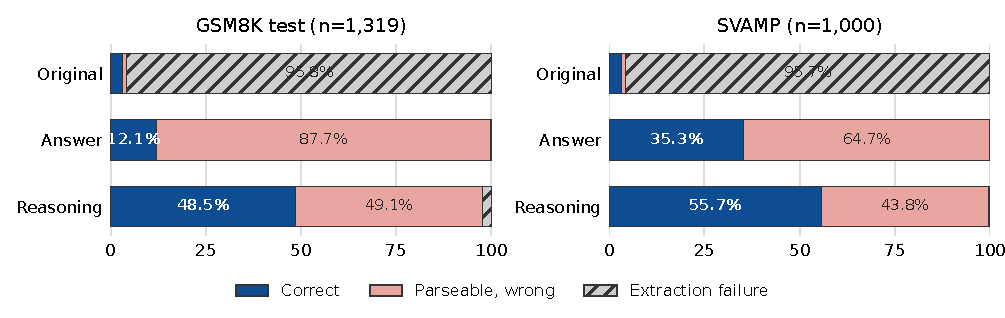
\includegraphics[width=\textwidth]{../figures/outcome_decomposition.pdf}
\caption{Required test predictions by outcome. Each bar sums to 100\%: correct ($C$), parseable but wrong ($E-C$), or extraction failure ($N-E$), computed from the six recorded \texttt{scores.csv} rows.}
\label{fig:outcomes}
\end{figure*}

The original model's strict-format scores are dominated by extraction failures: 1,263/1,319 on GSM8K and 957/1,000 on SVAMP. The answer-only adapter leaves only 3 and 0 such failures, yet gives 1,157 and 647 \emph{parseable but incorrect} answers. It learns the requested line format much more reliably than the mathematics. Reasoning SFT has slightly lower extraction rates than answer-only, but produces 640 versus 159 correct GSM8K answers and 557 versus 353 correct SVAMP answers. Among questions where \emph{both} tuned models yield a parseable answer, reasoning still wins 640 to 158 on GSM8K ($n=1{,}285$) and 557 to 352 on SVAMP ($n=995$). Its numerical advantage survives control for format compliance.

Paired examples reveal the cost as well as the benefit of worked-solution supervision. From Answer to Reasoning, 534 GSM8K predictions change from wrong to correct and 53 from correct to wrong, a net gain of 481; SVAMP changes are 276 and 72, a net gain of 204. These are paired counts on the same ordered questions, not a comparison of different samples.

\begin{table}[t]
\centering
\scriptsize
\setlength{\tabcolsep}{3pt}
\begin{tabular}{@{}lrrrr@{}}
\toprule
Adapter & Train 1/2 & Val. 1/2 & Min. & GiB \\
\midrule
Answer & 0.675/0.518 & 0.646/0.635 & 10.70 & 5.17 \\
Reasoning & 0.372/0.299 & 0.359/0.360 & 11.18 & 7.89 \\
\bottomrule
\end{tabular}
\caption{Required two-epoch training histories, rounded from the recorded log files. Losses average training/validation batches; peak memory is the training-run GPU maximum.}
\label{tab:training}
\end{table}

Training histories (Table~\ref{tab:training}) show decreasing training loss in both runs. Answer-only validation loss also falls, while reasoning validation loss is almost unchanged between epochs. Losses across target formats are not directly comparable because one target is a number and the other a worked solution. I retain both specified two-epoch checkpoints; neither test set selects an epoch.

\section{Controlled extensions}
\paragraph{Prediction-level error analysis.} Four cases from the unchanged prediction files (Table~\ref{tab:cases}) separate success, valid-answer errors, extraction failures, and cross-dataset regressions. On GSM8K 462, all three answers parse, but Answer returns 75 rather than $21+100/2=71$. On GSM8K 1085, Original calculates $(8/4)\times13=26$ and then writes after the final marker, so its answer is rejected; Reasoning instead omits division by four and returns 104. On SVAMP 605, Original computes $81\times33=2673$ without the marker, whereas Reasoning sets up the multiplication but evaluates it as 2559. On SVAMP 838, Original correctly reconstructs $17+9+8=34$ while both adapters return 26. Average gains therefore coexist with specific regressions, including on the external set.

\begin{table}[t]
\centering
\scriptsize
\setlength{\tabcolsep}{3.2pt}
\begin{tabular}{@{}lrrrr@{}}
\toprule
Example & Gold & Original & Answer & Reasoning \\
\midrule
GSM8K 462 & 71 & 71 C & 75 W & 71 C \\
GSM8K 1085 & 26 & 26 F & 26 C & 104 W \\
SVAMP 605 & 2673 & 2673 F & 2679 W & 2559 W \\
SVAMP 838 & 34 & 34 C & 26 W & 26 W \\
\bottomrule
\end{tabular}
\caption{Representative saved outputs: C = correct, W = wrong but parseable, F = extraction failure. A number beside F appears in the raw text but fails the required parser. IDs are \texttt{gsm8k-00462}, \texttt{gsm8k-01085}, \texttt{chal-605}, and \texttt{chal-838}; each was selected from an observed outcome category by shortest question, then ID.}
\label{tab:cases}
\end{table}

\paragraph{Capacity and decoding budget.} The capacity variant doubles LoRA rank from 8 to 16 and alpha from 16 to 32, holding alpha/rank at 2 and all other training settings fixed. Trainable parameters rise from 10.46M to 20.92M. On the same fixed 200-example GSM8K validation slice, accuracy is 55.5\% versus 53.5\% for required rank 8; on full tests it falls to 47.69\% GSM8K and 53.20\% SVAMP, both below rank 8. This comparison changes rank and alpha jointly, so it tests capacity at fixed scaling rather than rank alone. Extending greedy output from 256 to 512 tokens on the fixed validation slice raises rank-8 reasoning accuracy from 53.5\% to 54.5\% and extraction from 97.5\% to 100\%; answer-only accuracy stays at 15.0\%. The extra-token check is exploratory and leaves the required 256-token test protocol intact.

\paragraph{Training-target cleaning.} I strip GSM8K calculator annotations of the form \verb|<<...>>| from training solutions only, keeping the prose, arithmetic, and final answer. This changes 6,641/6,725 targets and removes 21,398 annotations; validation and test data remain unchanged. Accuracy becomes 48.60\% GSM8K and 52.20\% SVAMP. The GSM8K change is +0.08 points and the SVAMP change is $-3.50$ points relative to required Reasoning. Cleaning raises format extraction on GSM8K from 97.65\% to 99.70\% but does not improve transfer accuracy.

\paragraph{External data and volume control.} MathQA \citep{amini2019mathqa} supplies 2,000 additional training items selected from its training split. I retain questions with a unit-free numeric answer matching a supported arithmetic program, remove answer options and the source rationales, derive a calculation trace from the annotated program, and append the same final-answer line. Filtering leaves 3,440 eligible unique items from 29,837 source training rows. A protected pool of 9,792 supplied GSM8K/SVAMP questions is screened by normalized exact match, number-masked match, token-set similarity, and word trigrams; no selected item meets an overlap threshold. The control appends 2,000 distinct, seeded repeats from the permitted GSM8K training set. Both variants contain 8,725 training examples, use two epochs and the rank-8 settings, and start from the same frozen base. Example count and optimizer updates are thus matched.

\begin{table}[t]
\centering
\footnotesize
\setlength{\tabcolsep}{2pt}
\begin{tabular}{@{}lrrrr@{}}
\toprule
Reasoning condition & Train $n$ & Val$_{200}$ & GSM8K & SVAMP \\
\midrule
Required rank 8 & 6,725 & 53.50 & 48.52 & 55.70 \\
Rank 16 & 6,725 & 55.50 & 47.69 & 53.20 \\
Clean targets & 6,725 & 56.50 & 48.60 & 52.20 \\
Repeat control & 8,725 & 58.50 & 43.75 & 52.10 \\
MathQA mixture & 8,725 & 54.00 & 47.92 & 55.90 \\
\bottomrule
\end{tabular}
\caption{Extension accuracy (\%). Rank 16 uses alpha 32. Val$_{200}$ is the same exploratory 200-question GSM8K validation slice for all rows; full test sets have 1,319 and 1,000 items. Required rank-8 test scores come from the original main run.}
\label{tab:optional}
\end{table}

Under matched example counts, the MathQA mixture exceeds repetition by 4.17 GSM8K and 3.80 SVAMP points (Table~\ref{tab:optional}). Against the original required Reasoning run, it is 0.61 points lower on GSM8K and 0.20 points higher on SVAMP. The 200-example validation ranking does not predict the full GSM8K ranking: repetition leads on the validation slice but performs worst on the test set. The required adapter remains the prespecified main comparison.

\section{Interpretation and limits}
Worked-solution targets produce a much stronger strict-format solver than answer-only targets on both datasets. The conditional and paired comparisons locate much of that gain in numerical correctness; the answer-only adapter's main strength is near-perfect format compliance. The original model's 3\% strict-format baseline is chiefly an output-format result, since the parser rejects most outputs without a final marker. Its conditional accuracy describes only the small, selected subset that complied, not all of its mathematical reasoning.

The extension comparisons have three boundaries. First, the runs use one training seed and the 200-question slice is exploratory; the full-test results were inspected, not used for a new model-selection rule. Second, equal example counts do not equalize total target-token exposure across MathQA and repeated GSM8K. Third, lexical decontamination cannot rule out semantic paraphrases or numerically plausible but incorrect MathQA programs. These points limit attribution of the mixture's observed advantage over repetition, while leaving the saved exact-match results intact.

\section{Conclusion}
The required Reasoning adapter reaches 48.52\% GSM8K and 55.70\% SVAMP, versus 12.05\% and 35.30\% for Answer. The four extensions add a narrower result: more adapter capacity and calculator-annotation cleaning do not improve both tests, whereas filtered external questions help relative to an equal-size repetition control. The original experiment notebook's 24 code cells ran successfully, and the required metrics were recomputed from all 6,957 saved prediction rows. Replicated runs and a stronger semantic overlap audit would test the stability of the external-data comparison.

\bibliographystyle{plainnat}
\bibliography{references}

\end{document}
